% PANORAMICA DEGLI UCS: 3, 4, 5, 6, 7, 8
\newpage
\subsubsection{Panoramica della gestione di un'organizzazione}%kite level
La seguente figura illustra le azioni possibili per i vari amministratori dopo aver selezionato un'organizzazione\ap{G} [UCS 3].
\begin{figure}[h]
	\centering
    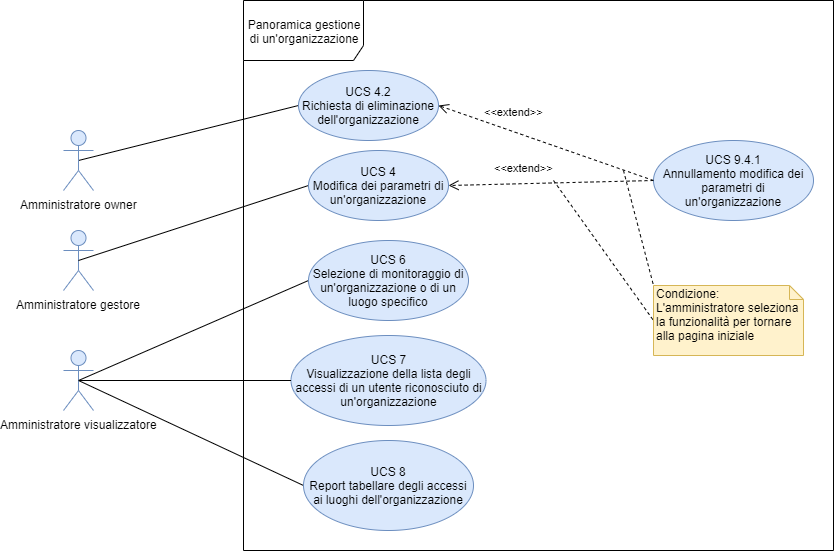
\includegraphics[scale=0.53]{sezioni/UseCase/Immagini/Panoramica gestione organizzazione.png}
    \caption{Panoramica della gestione di un'organizzazione\ap{G}}
\end{figure}